% =====================================================================================
% Document : rendu du DM2
% Auteur : Xavier Gandibleux
% Année académique : 2018-2019

\section*{Livrable du devoir maison 3 : \\ Battle of metaheuristics}

%
% -----------------------------------------------------------------------------------------------------------------------------------------------------
%

\vspace{5mm}
\noindent
\fbox{
  \begin{minipage}{0.97 \textwidth}
    \begin{center}
      \vspace{1mm}
        \Large{Présentation succincte des choix de mise en \oe uvre de la métaheuristique concurrente à GRASP appliquée au SPP}
      \vspace{1mm}
    \end{center}
  \end{minipage}
}
\vspace{2mm}


%\prof{Présenter l'algorithme mis en oeuvre. Illustrer sur un exemple didactique (poursuivre avec l'exemple pris en DM1). Présenter vos choix de mise en oeuvre.}

Nous avons choisi d'implémenter les méthodes de recherche Tabou (TS) et de Recuit Simulé (SA). 
Nous présentons donc chacune des deux méthodes dans les paragraphes suivants :

\paragraph{Recherche Tabou}

Rappel de la méthode :

La méthode Tabou, ou Tabu Search, est une méthode déterministe de recherche d'optimum. L'idée est de chercher la meilleure solution possible d'un problème(ici un SPP) en parcourant l'ensemble des solutions, sans rester bloqué dans un optimum local comme pour une plus profonde descente. Cela signifie donc avancer dans l'espace des solutions sans pouvoir immédiatement revenir en arrière. \\
Pour démarrer, l'algorithme part d'une solution admissible et cherche son meilleur voisin. (Cette démarche s'applique même si le voisin trouvé est moins bon que la solution actuelle). Une fois le meilleur voisin trouvé, le mouvement réalisé est enregistré comme mouvement tabou, c'est-à-dire inutilisable pour une certaine période de temps (un nombre de tours de boucles dans les faits). Ce meilleur voisin est ensuite comparé avec la meilleure solution trouvée jusqu'à maintenant, et la meilleure des deux est gardée en mémoire. On se place ensuite sur le meilleur voisin trouvé pour inspecter son voisinage. La même démarche que précédemment sera prise, avec ceci près que le meilleur voisin trouvé ne devra pas être atteint avec un mouvement actuellement tabou. Au fur et à mesure que l'algorithme se déroule, le nombre de mouvement inutilisable augmente. Pourtant, cela pourrait empêcher de revenir sur des solutions qui ont été vu mais qui permettent de passer sur une partie de l'espace des solutions non visitée. Pour cette raison, il existe un temps ou nombre de boucles au bout desquels un mouvement redevient utilisable.\\
Dans cette méthode, la liste/tableau de mouvement Tabou est l'élément essentiel pour permettre de se déplacer dans une grande partie de l'espace des solution et d'éviter de retomber dans un optimum local déjà visité au prochain tour de boucle. La meilleure solution sera donc celle retenue lors du parcours de l'espace des solutions, à l'issue d'un nombre d'itérations ou temps limite.

Une amélioration de l'algorithme Tabu Search, nommé Reactive TS, est de faire varier la longueur de la liste tabou, ou autrement dit la durée d'interdiction d'un mouvement en fonction d'un apprentissage sur les données.
En effet, il est possible de voir l'algorithme boucler et rester dans une même partie de l'espace parce qu'il ne peut en sortir pour cause de mouvements tabous. L'idée est donc de détecter ces cas et d'autoriser à nouveau ces mouvements, pour sortir de ce cyclage.



Implémentation :

Toujours en utilisant la structure de données avec les vecteurs de vecteurs, nous avons aussi repris deux fonctions du DM1:
\begin{itemize}
    \item le glouton déterministe le plus efficace (gloutonVxV)
    \item la plus profonde descente, où l'on incorpore la notion de mouvement tabou (pour la version 2 du tabou)
    \item la fonction d'admissibilité
\end{itemize}

Dans l'implémentation du calcul des voisins, nous avons choisis, pour des raison d'efficacité, de parcourir les voisins en retenant le plus petit au fur et à mesure au lieu de calculer l'ensemble des voisins puis de choisir le plus petit.


Remarques :

Dans un premier temps, nous avions choisi, pour optimiser le temps d'exécution, de représenter la liste tabou dans une matrice (dans l'idéal, cette matrice serait triangulaire). Nous n'utilisions alors qu'un mouvement d'1-1 échange. Cependant, pour les instances qui ont des fonctions objectifs avec des coûts tous similaires, cela ne permet aucune amélioration. Nous avons donc réalisé une seconde implémentation.

Seconde implémentation (tabou3) :

Pour améliorer notre tabou, nous avons décidé d'augmenter son voisinage en ajoutant les 2-1 et 0-1 échanges. Nous avons donc repris les échanges utilisés par le grasp en y ajoutant la notion de mouvements tabou.

Ce nouveau voisinage permet de mieux explorer l'espace des solution mais en contrepartie, nous avons une représentation des mouvements tabou moins précise. En effet, dans notre liste (représentée dans un tableau pour une question d'efficacité), nous ne retenons que les variables qui ont récemment été mise à 1. Cela ne correspond pas à un mouvement mais à cause de l'ajout des nouveaux voisinages, la représentation de la liste tabou pouvait devenir très lourde. Nous avons donc choisi de la rendre moins précise.

Ce choix a pour effet qu'un tabou représente plusieurs mouvements possibles et donc peut potentiellement empêcher un mouvement inédit améliorant.


\paragraph{Recuit simulé}

Rappel de la méthode :

Le Recuit Simulé est une méthode stochastique qui recherche le meilleur voisin possible mais en contrôlant au fur et à mesure la direction de recherche dans l'espace des solutions.

Le Recuit Simulé consiste à se déplacer aléatoirement dans un voisinage en acceptant parfois certaines solutions détériorantes afin de ne pas rester coincé dans un voisinage. Ce contrôle se fait en utilisant un schéma de refroidissement : une fonction simulant le refroidissement d'un alliage est utilisée. Cette fonction décroit exponentiellement.
Le principe est le suivant : à partir d'une solution, on choisit au hasard l'un de ces voisins admissibles. Un nombre p est tirée au hasard entre 0 et 1. La solution voisine S' est retenue si la solution est améliorante ou bien si le nombre p est inférieur à la fonction de refroidissement (qui varie en fonction de la température et de la différence entre la meilleure solution et l'actuelle). Si la solution est acceptée, on la compare ensuite avec la meilleure solution en mémoire. Sinon, on garde la solution S. Enfin, la température T est mise à jour. Cette démarche se répète ensuite sur la solution retenue jusqu'à une limite de temps ou bien un certain nombre de voisins refusés.

Implémentation :

Nous avons remarqué qu'utiliser un seul swap comme voisinage était une mauvaise idée, car toutes les instances à fonction objectif composées uniquement de coûts réduits à 1 ne peuvent pas être améliorées. Nous avons donc élargi le voisinage de la manière suivante :
Le voisinage choisi oscille aléatoirement entre un 1-1échange, un 0-1 et un 1-0 à respectivement 80\%, 10\%,et 10\% de chance.
De cette manière, l'algorithme ne reste pas bloqué sur les instances à fonction objectifs spéciales ou tout autre voisinage avec une configuration complexe.


Dans cette méthode, il y a donc 3 (voire 4) paramètres à régler :
\begin{itemize}
    \item la température $ T_0 $ : En partant au début d'une température très grande, on décide d'accepter beaucoup de solution dégradante pour ensuite être de plus en plus restrictifs au fur et à mesure que cette température baissera.
    \item le palier L : On note que la mise à jour de la température se fait en fonction de la température initiale $ T_0 $ mais aussi de la taille du palier donnée en entrée. Un palier très long est plus longtemps permissif envers les solutions de mauvaises qualités.
    \item Le coefficient de refroidissement $ \alpha $ : Ce coefficient est celui qui permet de régler la vitesse de convergence de la fonction de refroidissement vers 0. 
    \item Le nombre de refus maximal autorisé (éventuel critère limite): Dans notre cas, pour pouvoir comparer avec le TS avec une même contrainte de temps, nous avons peu joué dessus.
\end{itemize}


%
% -----------------------------------------------------------------------------------------------------------------------------------------------------
%

\vspace{5mm}
\noindent
\fbox{
  \begin{minipage}{0.97 \textwidth}
    \begin{center}
      \vspace{1mm}
      \Large{Expérimentation numérique comparative \\
        Reactive GRASP + Path Relinking VS Recherche Tabou VS Recuit Simulé}
      \vspace{1mm}
    \end{center}
  \end{minipage}
}
\vspace{2mm}

%\prof{\noindent Présenter le protocole d'expérimentation (environnement matériel; budget de calcul; condition(s) d'arrêt; réglage des paramètres).}

Les conditions pour les expérimentations sont les suiavntes : 
Les codes sont réalisés sous Julia 0.6.4 en mode mutlicoeur avec la commande : julia -p $<$nombres de coeurs$>$

L'ensemble des programmes ont été réalisé en julia 0.6.4 et les tests ont été effectués avec un pc acer sous ubuntu18 avec les caractéristiques suivantes : 
\begin{itemize}
\item RAM : 4 Gio
\item CPU : Intel® Core™ i3-7130U CPU @ 2.70GHz × 4 
\item GPU : Intel® HD Graphics 620 (Kaby Lake GT2)
\end{itemize}


\paragraph{Protocole}
Des tests sont réalisées avec les deux méthodes Tabu Search, Simulated Annealing et sont comparées aux résultats du ReactiveGrasp.
Pour chaque instance, on lance des tests avec chaque méthode, et en essayant avec deux temps limites possibles 3 et 10 secondes.


%\prof{Rapporter graphiquement vos résultats selon $\hat{z}_{min}$, $\hat{z}_{max}$, $\hat{z}_{moy}$ mesurés à intervalles réguliers (exemple de pas de 10 secondes).}
\begin{example}
  Une éxecution du Recuit Simmulé
  \begin{figure}[htb!]
    \centering
    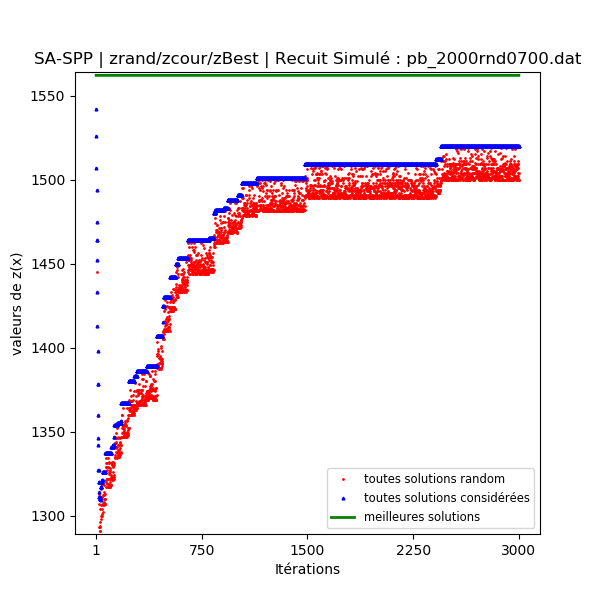
\includegraphics[scale=0.5]{fig/recuit.png}
    %\caption{patate}
    \label{fig:recuit}
  \end{figure}
\end{example}

\begin{example}
  Une éxecution de la Recherche Tabou
  \begin{figure}[htb!]
    \centering
    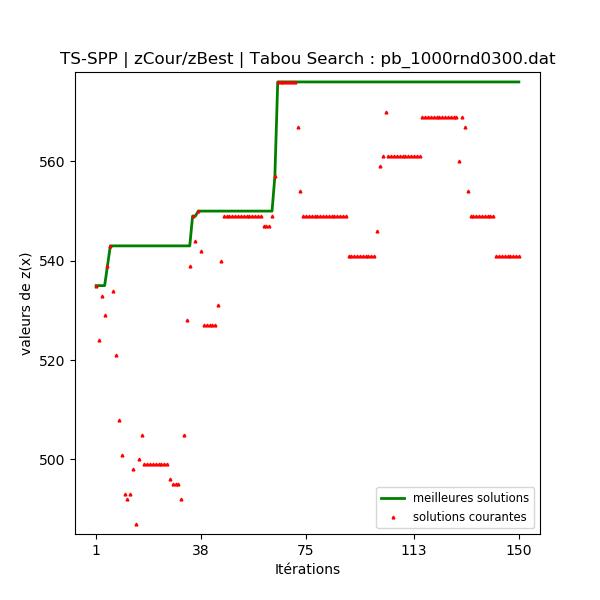
\includegraphics[scale=0.5]{fig/tabou.png}
    %\caption{patate}
    \label{fig:recuit}
  \end{figure}
\end{example}

On observe que globalement, nos solutions obtenues par les gloutons et servant de solution de départ pour les autres méthodes sont de bonne qualité. C'est pour cette raison que le recuit simulé a du mal à l'améliorer dans l'exemple ci-dessus. En fait, cela est aussi vrai pour plusieurs instances, les TS et SA n'arrive pas toujours à améliorer car la solution de départ est très bonne.


%\prof{Rapporter l'étude de l'influence du paramètre $\alpha$.}
Paramétrage du Tabu Search : Lorsque la tabou liste est longue, si on tombe dans une phase de cyclage (c'est-à-dire un cas où il est difficile de sortir d'une partie du voisinage), elle donne l'occasion d'en sortir. A l'inverse, si elle est courte, il y a le risque de cycler et de rester dans la même zone indéfiniment. On remarque qu'une tabou liste de taille 25 est un bon compromis pour éviter le cyclage et en même temps parcourir l'ensemble de l'espace. Bien sûr, ce réglage correspond au voisinage que nous avons choisi.

Paramétrage du Simulated Annealing : Nous avons étudié les trois paramètres sur toutes les instances. Nous en donnons un exemple ici, sur l'instance : 1000rnd0700
Le paramétrage de référence : L = 6, $T_0$ = 150, $\alpha$ = 0.4
On part d'un glouton à 92.83\% de la solution.
\begin{center}
    \begin{tabular}{|c|c|c|c|}  
    \hline
    paramètre changé & sa valeur & Qualité de solution &  Observations générales \\
     \hline
     ... & ...  & 94.64\% & référence\\
     \hline
     L & 3 & 93.05\% & descente trop rapide pour tomber sur une bonne solution\\
     \hline
     L & 10 & 92.83\% & affinage ralenti, très peu de restriction\\
     \hline
     $T_0$ & 50 & 93.1\% & pas assez de liberté\\
     \hline
     $T_0$ & 500 & 94.25\% & trop de temps à refroidir\\
     \hline
     $\alpha$ & 0.9 & 92.83\% & pas assez agressif \\
     \hline
     $\alpha$ & 0.15 & 94.56\% & convergence trop rapide \\     
     \hline
   \end{tabular}
\end{center}

Concernant le paramètre $T_0$ , ces observations dépendent aussi du temps/nombre d'itérations limite accordées. En effet, une chaleur très élevée peut donner de bons résultats si on lui donne beaucoup de temps pour refroidir et arriver dans la phase de restrictions des solutions.
On note cependant que le paramétrage pourrait être meilleur, en prenant en compte, par exemple, du nombre de variables et de contraintes de l'instance sur laquelle la méthode est appliquée.

%\prof{Présenter sous forme de tableau les résultats finaux obtenus pour les 10 instances sélectionnées.}

\begin{center}
    \begin{tabular}{|c|c|c|c|c|}  
    \hline
    nom de l'instance &  Tabou Search & Simmulated Annealing & Reactive Grasp\\
     \hline
     pb1000rnd0300 & 87.14\% & 79.43\% & 85.17\% \\
     \hline
     pb1000rnd0700 & 95.22\% & 93.67\% & 94.65\% \\
     \hline
     pb100rnd0500 & 97.97\% & 97.97\% & 100\% \\
     \hline
     pb2000rnd0700 & 90.83\% & 87.58\% & 91\% \\
     \hline
     pb200rnd0100 & 94.95\% & 88.22\% & 96.88\% \\
     \hline
     pb200rnd0300 & 95.9\% & 94.25\% & 96.72\% \\
     \hline
     pb200rnd0700 & 96.81\% & 95.12\% & 99.4\% \\
     \hline
     pb200rnd0900 & 99.55\% & 99.55\% & 99.92\% \\
     \hline 
     pb500rnd0700 & 97.63\% & 97.11\% & 98.69\% \\
     \hline 
     pb500rnd0900 & 98.39\% & 99.15\% & 98.79\% \\
     \hline
    \end{tabular}
\end{center}

Paramètres sur 3 sec :
\begin{itemize}
\item R-Grasp : $N_{\alpha} = 10$ et $V_{\alpha} = [0.35,0.5,0.65,0.8,0.95]$
\item TS : Tabou lenght = 25
\item SA : L = 6, $T_0$ = 150, $\alpha$ = 0.4
\end{itemize}

On peut comparer les heuristiques en comptant le nombre de fois où elles ont obtenues un meilleur résultat, pour un même temps donné. Cependant, il ne faut pas oublier que les solutions trouvées par ces trois méthodes restent assez proches. Nous remarquons que les méthodes aléatoires peuvent occasionnellement dépasser les solutions du Tabou Search. Ainsi, nous pouvons noter que le Tabu Search, en une fois nous permet de trouver une très bonne solution. Cependant, avec plusieurs tentatives et un bon tuning de paramètres, comme pour le Grasp, il devient possible de trouver des solutions encore meilleures mais de manière beaucoup plus coûteuse. 
\begin{center}
  Médailles pour les dix instances : \\
    \begin{tabular}{|c|c|c|c|}  
    \hline
    heuristique & ---Or--- & ---Argent--- & ---Bronze---\\
    \hline
    TABOU & 3 & 7 & 3 \\
    \hline
    SA    & 1 & 3 & 9\\
    \hline
    GRASP & 7 & 3 & 1\\
    \hline
    \end{tabular}
\end{center}

Des tests sont lancés pendant 3 et 10 secondes avec une TL de 10 sans remarquer de différences dans les solutions. La version ci-dessous correspond à des tests avec un temps limite de 3 secondes. Nous remarquons que Grasp est le meilleur sur ce groupe d'instances. Cela s'explique par l'apprentissage  du paramètre $\alpha$ et l'ajout du path-relinking. Les deux autres méthodes méritent encore quelques modifications pour les parfaire. Pour le Tabu Search, il serait bon de réaliser une implémentation non pas avec une matrice des variables changées mais bien une liste de mouvements. Pour le Simulated Annealing, il serait possible d'améliorer les résultats avec un tuning des paramètres en prenant en compte le nombre de variables et de contraintes. Il est aussi important de noter que les méthodes aléatoires dépendent des graines choisies et, on peut se demander si, selon celles choisies, il peut-être possible de tomber plus facilement sur une solution meilleure que celle du Tabu Search par hasard. En effet, plusieurs tentatives avec les mêmes paramètres avec le SA ont montré qu'il était possible de dépasser occasionnellement le Tabu Search. \\
Dans un test sur l'ensemble des instances, on remarque que le TS a autant de succès que le ReactiveGrasp, et le SA donne aussi de bons résultats. Respectivement, ces méthodes détiennent les meilleures solutions pour 38, 39 et 21 instances. Nous pouvons nous demander si chaque méthode est bonne pour un type de sous-problème donné. 

%
% -----------------------------------------------------------------------------------------------------------------------------------------------------
%

\vspace{5mm}
\noindent
\fbox{
  \begin{minipage}{0.97 \textwidth}
    \begin{center}
      \vspace{1mm}
        \Large{Discussion}
      \vspace{1mm}
    \end{center}
  \end{minipage}
}
\vspace{2mm}


%\prof{Tirer des conclusions en comparant les résultats collectés avec vos deux métaheuristiques.}
Conclusion globale :

En remarque globale, on observe que le choix du voisinage est primordial pour l'efficacité d'une heuristique sur un problème. Nous remarquons aussi qu'une heuristique prise pour un type de (sous-)problème est plus optimisé et donne de meilleurs résultats. En effet, nos premières tentatives de TS et SA étaient bonnes pour des instances avec des fonctions objectifs avec des coûts réduits non tous égaux à 1. Nous pouvons remarquer que l'heuristique TS a l'avantage de donner dès le premier lancement une solution de bonne qualité en général, alors que celles stochastiques nécessitent un paramétrage.

Pistes d'améliorations :

Comme noté précédemment, nous supposons que les deux heuristiques TS et SA peuvent encore être améliorées, via ,respectivement, une liste des mouvement et un apprentissage des paramètres par rapport aux nombres de variables et de contraintes notamment. 

Comme amélioration, nous avons essayé de faire un path-relinking sur les solutions du TS et du SA puis un deuxième entre cette nouvelle solution et celle du reactive grasp. De cette manière, nous espérions construire une très bonne solution mais malgré plusieurs tests avec plusieurs temps d'arrêts différents, nous n'avons pas observé d'amélioration.

Il pourrait aussi être intéressant d'essayer de trouver un moyen pour avoir une borne nous indiquant l'optimalité à une erreur près. 


%\prof{Quelles sont les recommandations que vous émettez à l'issue de l'étude ?}

L'optimisation des heuristiques se fait à tous les niveaux : sur les structures de données, sur les caractéristiques du langage, et sur une l'implémentation intelligente de l'algorithme en évitant toutes opérations coûteuses. On remarque vite l'avantage d'une heuristique déterministe pour l'analyse des résultats. Afin d'obtenir une solution de bonne qualité, il est important de bien choisir une heuristique adaptée au problème, et de bien analyser les différents types d'instances à résoudre.





